\documentclass{article}

\usepackage{graphicx}
\usepackage{tikz}
\usepackage{tikzsymbols}
\usetikzlibrary{calc,patterns,shapes.geometric}
\pagestyle{empty}
\usepackage[margin=0pt]{geometry}
\geometry{papersize={14in,12in}}

\def\centerarc[#1](#2)(#3:#4:#5){\draw[#1] ($(#2)+({#5*cos(#3)},{#5*sin(#3)})$) arc (#3:#4:#5);}

\begin{document}
	\begin{figure}
		\centering
		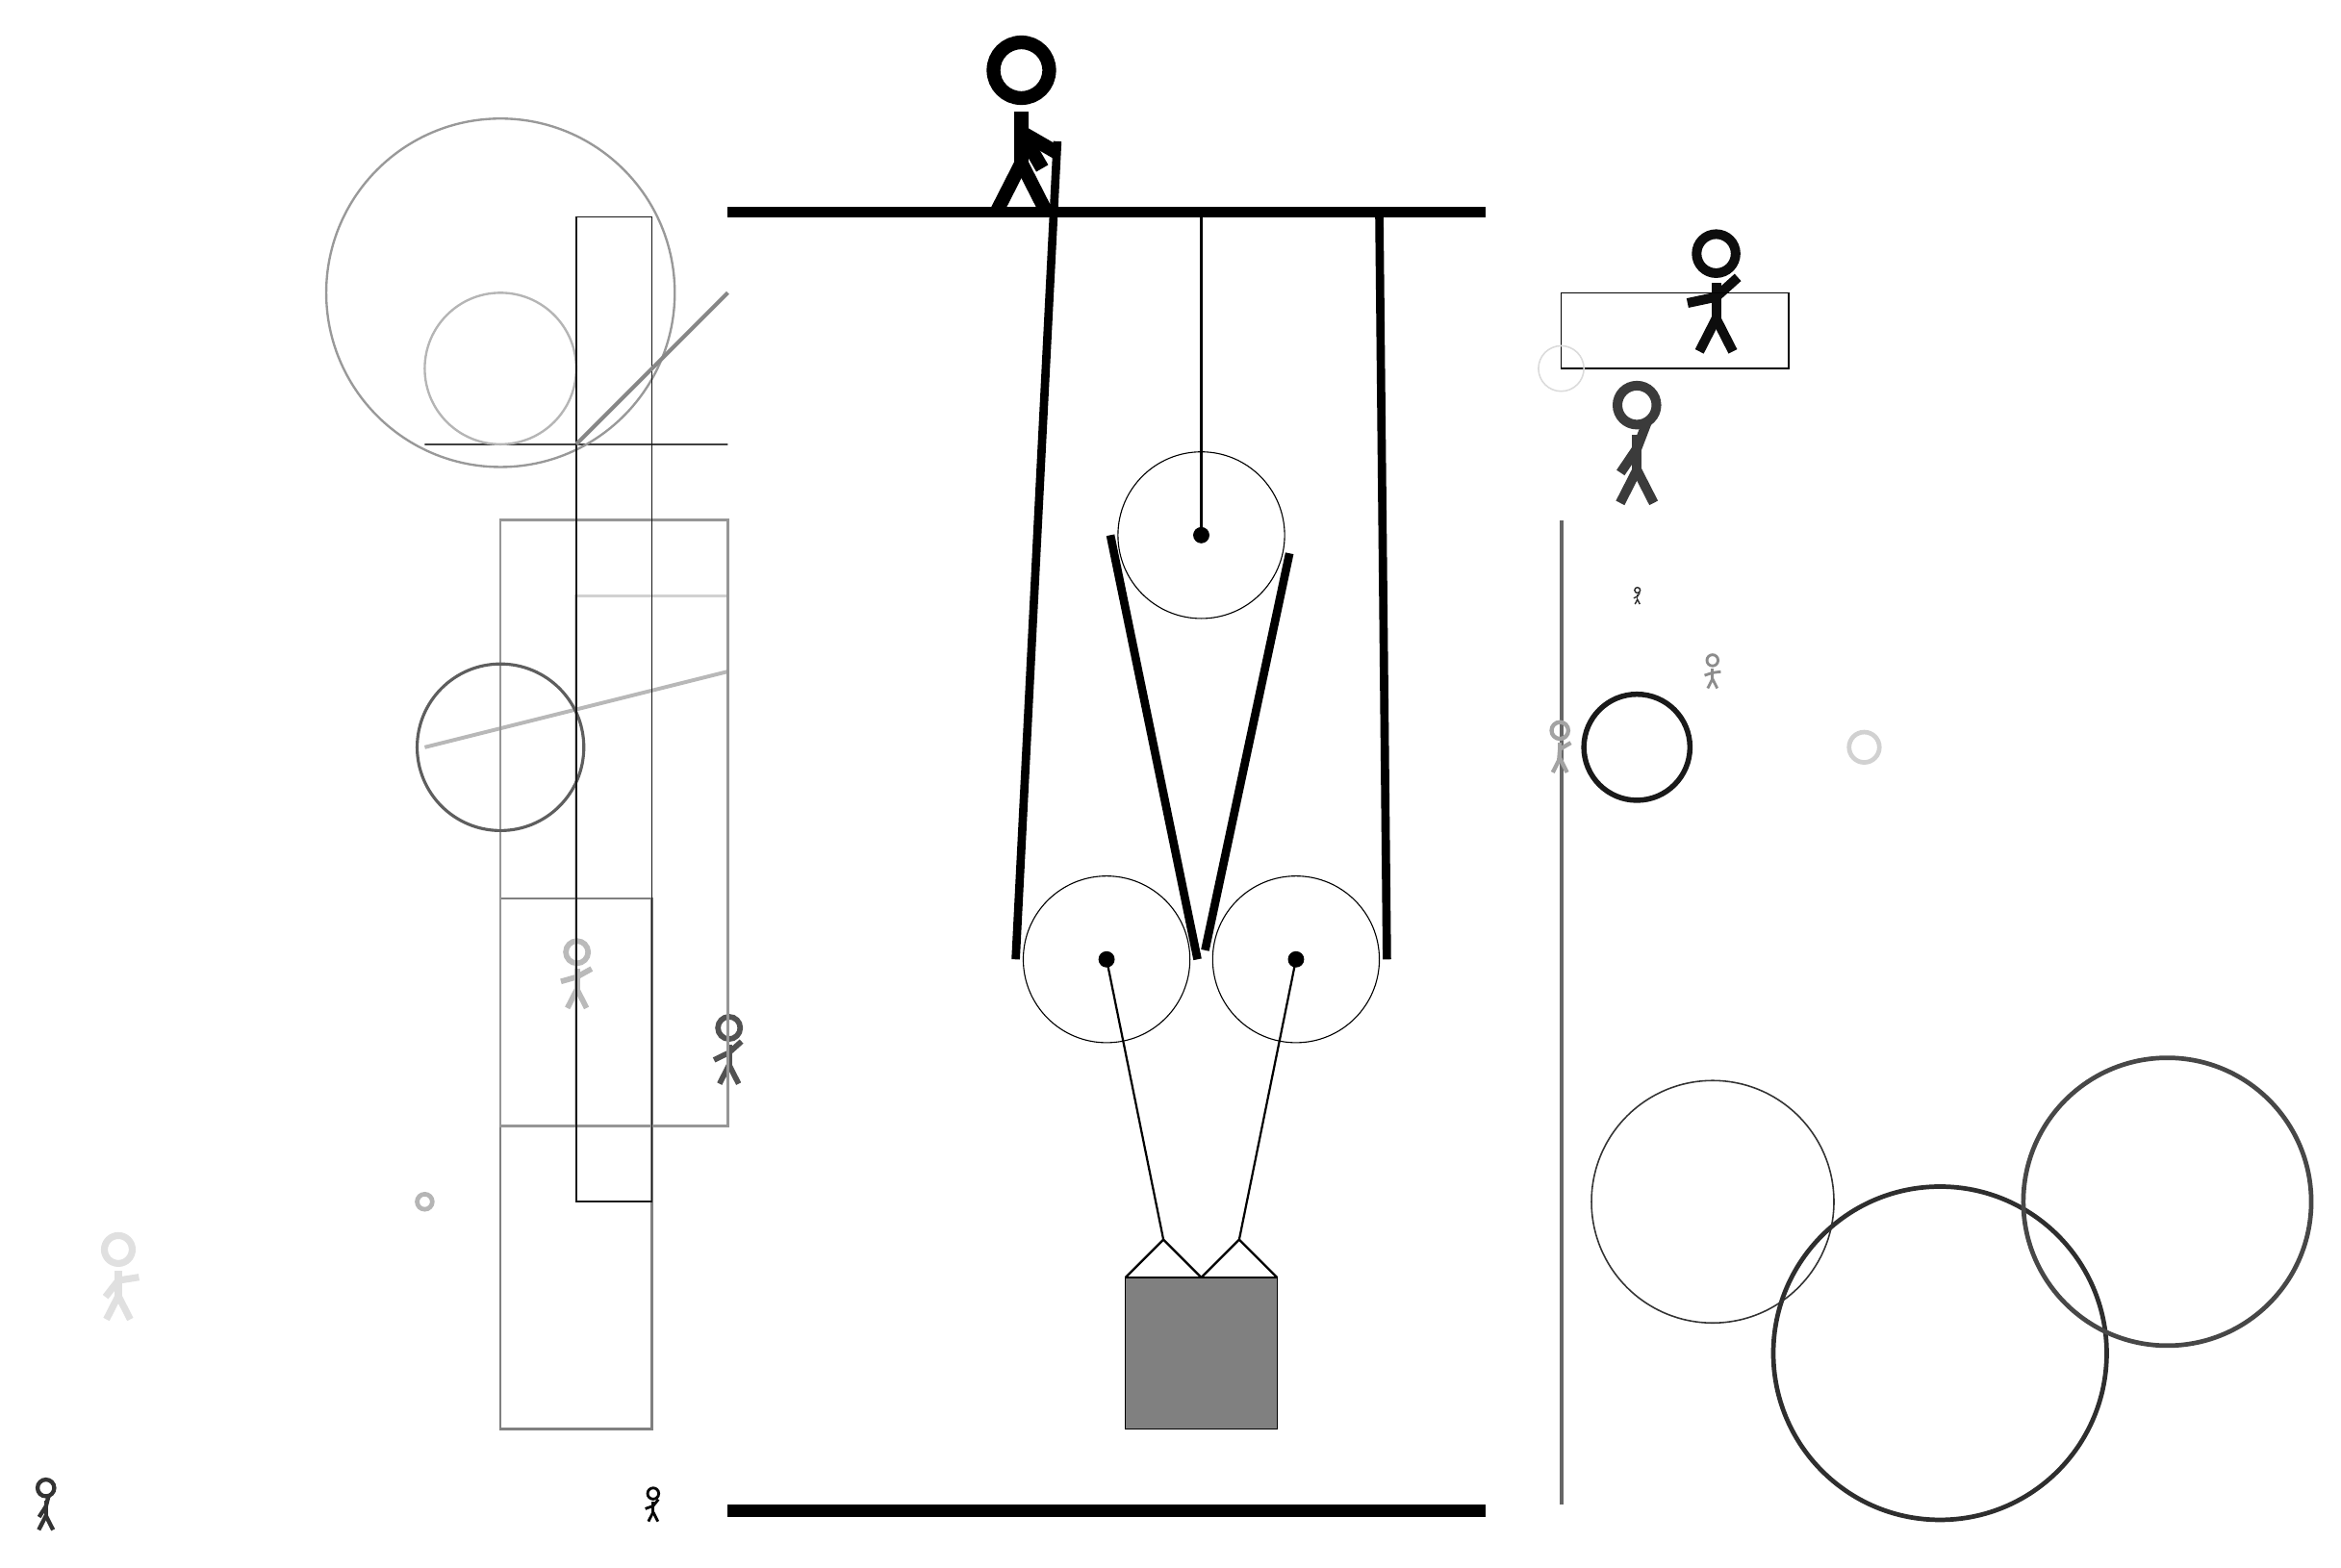
\begin{tikzpicture}
			%%%%% START %%%%%
			
			\draw[fill=black] (-4, 14) rectangle (6, 14.125);
			
			\draw (1, 4.2) circle (1.1);
			\draw[fill=black] (1, 4.2) circle (0.1);
			
			\draw[line width=0.2mm, color=black!75] (-4, 11) rectangle (-8, 11);
			
			\draw [line width=0.6mm, color=black!82](12, -1) circle (2.2);
			\draw [line width=0.6mm, color=black!18](11, 7) circle (0.2);
			\draw[line width=0.5mm, color=black!60](7, -3) -- (7, 10);
			
			\draw[line width=0.4mm, color=black!18] (-4, 2) rectangle (-6, 9);
			
			\node[line width=0.3mm, color=black!27] at (-6, 4) {\Strichmaxerl[4][16][29]};
			\node[line width=0.5mm, color=black!95] at (9, 13) {\Strichmaxerl[7][12][42]};
			
			\node[line width=0.7mm, color=black!77] at (8, 11) {\Strichmaxerl[7][56][69]};
			\node[line width=0.2mm, color=black!36] at (7, 7) {\Strichmaxerl[3][85][30]};
			
			\draw [line width=0.3mm, color=black!40](-7, 13) circle (2.3);
			\draw[line width=0.3mm, color=black!50] (-5, -2) rectangle (-7, 5);
			
			\node[line width=0.6mm, color=black!97] at (-5, -3) {\Strichmaxerl[2][20][51]};
			\draw [line width=0.3mm, color=black!29](-7, 12) circle (1.0);
			\node[line width=0.4mm, color=black!45] at (9, 8) {\Strichmaxerl[2][19][7]};
			\node[line width=0.6mm, color=black!83] at (8, 9) {\Strichmaxerl[1][26][57]};
			\node[line width=0.6mm, color=black!68] at (-4, 3) {\Strichmaxerl[4][26][42]};
			\draw [line width=0.6mm, color=black!29](-8, 1) circle (0.1);
			\draw[line width=0.5mm, color=black!28](-4, 8) -- (-8, 7);
			\draw[line width=0.3mm, color=black!41] (-4, 2) rectangle (-7, 10);
			\draw[line width=0.2mm, color=black!99] (7, 12) rectangle (10, 13);
			\draw [line width=0.2mm, color=black!80](9, 1) circle (1.6);
			
			\draw [line width=0.4mm, color=black!63](-7, 7) circle (1.1);
			\draw [line width=0.7mm, color=black!90](8, 7) circle (0.7);
			\draw[line width=0.2mm, color=black!91] (-5, 14) rectangle (-6, 1);
			\draw[line width=0.5mm, color=black!47](-6, 11) -- (-4, 13);
			
			\draw [line width=0.6mm, color=black!72](15, 1) circle (1.9);
			\draw [line width=0.2mm, color=black!14](7, 12) circle (0.3);
			\node[line width=0.3mm, color=black!12] at (-12, 0) {\Strichmaxerl[5][52][9]};
			\node[line width=0.3mm, color=black!80] at (-13, -3) {\Strichmaxerl[3][57][76]};
			
			\draw (2.25, 9.8) circle (1.1);
			\draw[fill=black] (2.25, 9.8) circle (0.1);
			\draw[thick] (2.25, 9.8) -- (2.25, 14);
			
			\draw (3.5, 4.2) circle (1.1);
			\draw[fill=black] (3.5, 4.2) circle (0.1);
			
			\draw[thick] (3.5, 4.2) -- (2.75, 0.5);
			\draw[thick] (1, 4.2) -- (1.75, 0.5);
			\draw[thick]  (1.25, 0) -- (1.75, 0.5) -- (2.25, 0);
			\draw[thick]  (2.25, 0) -- (2.75, 0.5) -- (3.25, 0);
			\draw[fill=black!50] (1.25, 0) rectangle (3.25, -2);
			
			\draw[line width=1.1mm] (0.35, 15) --  (-0.2, 4.2);
			\centerarc[line width=1.1mm](1, 4.2)(180:360:1.2000000000000002);
			\draw[line width=1.1mm] (2.2, 4.2) -- (1.05, 9.8);
			\centerarc[line width=1.1mm](2.25, 9.8)(-20:180:1.2000000000000002);
			\draw[line width=1.1mm](3.414, 9.56) -- (2.3, 4.32);
			\centerarc[line width=1.1mm](3.5, 4.2)(160:360:1.2000000000000002);
			\draw[line width=1.1mm](4.7, 4.2) -- (4.6, 14);
			
			\node at (-0.07, 15.2) {\Strichmaxerl[10][120][-30]};
			
			\draw[fill=black] (-4, -3) rectangle (6, -3.15);
			
			%%%%% END %%%%%
		\end{tikzpicture}
	\end{figure}	
\end{document}